\newpage
\section{Anhang}


\subsubsection{Messaufbau}



\begin{figure}[h]
    \centering
    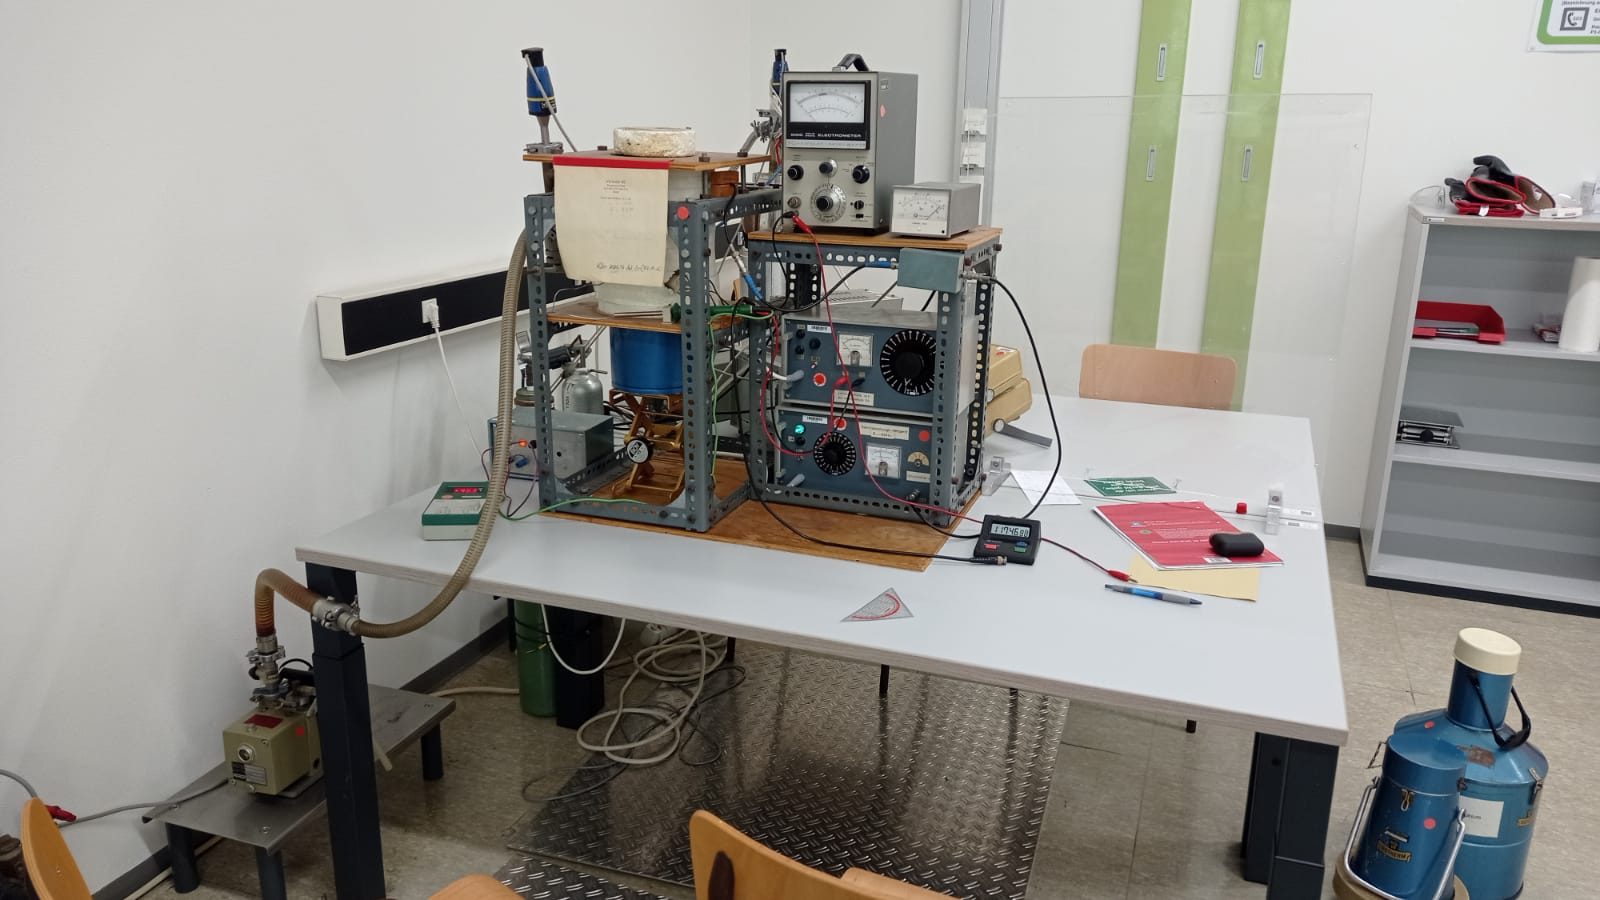
\includegraphics[width=0.7\textwidth]{latex/images/Aufbau.jpeg}
    \caption{Der Aufbau des Versuchs Dipolrelaxation.}
\end{figure}
%    \begin{table}[H]
%        \centering
%        \begin{tabular}{S [table-format=2.3] S [table-format=2.3] S [table-format=2.3] c }
%            \toprule
%            \multicolumn{1}{p{3.2cm}}{\centering$\text{Druck Messreihe 1 } $\\$ \text{in }\si{\milli\bar}$} &
%            \multicolumn{1}{p{3.2cm}}{\centering$\text{Druck Messreihe 2 } $\\$ \text{in }\si{\milli\bar}$} &
%            \multicolumn{1}{p{3.2cm}}{\centering$\text{Druck Messreihe 3 } $\\$ \text{in }\si{\milli\bar}$} &
%            \multicolumn{1}{p{3.2cm}}{\centering$\text{Druck gemittelt } $\\$ \text{in }\si{\milli\bar}$} \\
%            \midrule
%
%            \end{tabular}
%            \caption{Messwerte der Leckratenmessung für den Gleichgewichtsdruck $\SI{0.4}{\milli\bar}$ mit der Drehschieberpumpe.}
%            \label{tab:dreh_leck_1}
%    \end{table}


\subsection{Messwertfotos}

\begin{figure}[h]
    \centering
    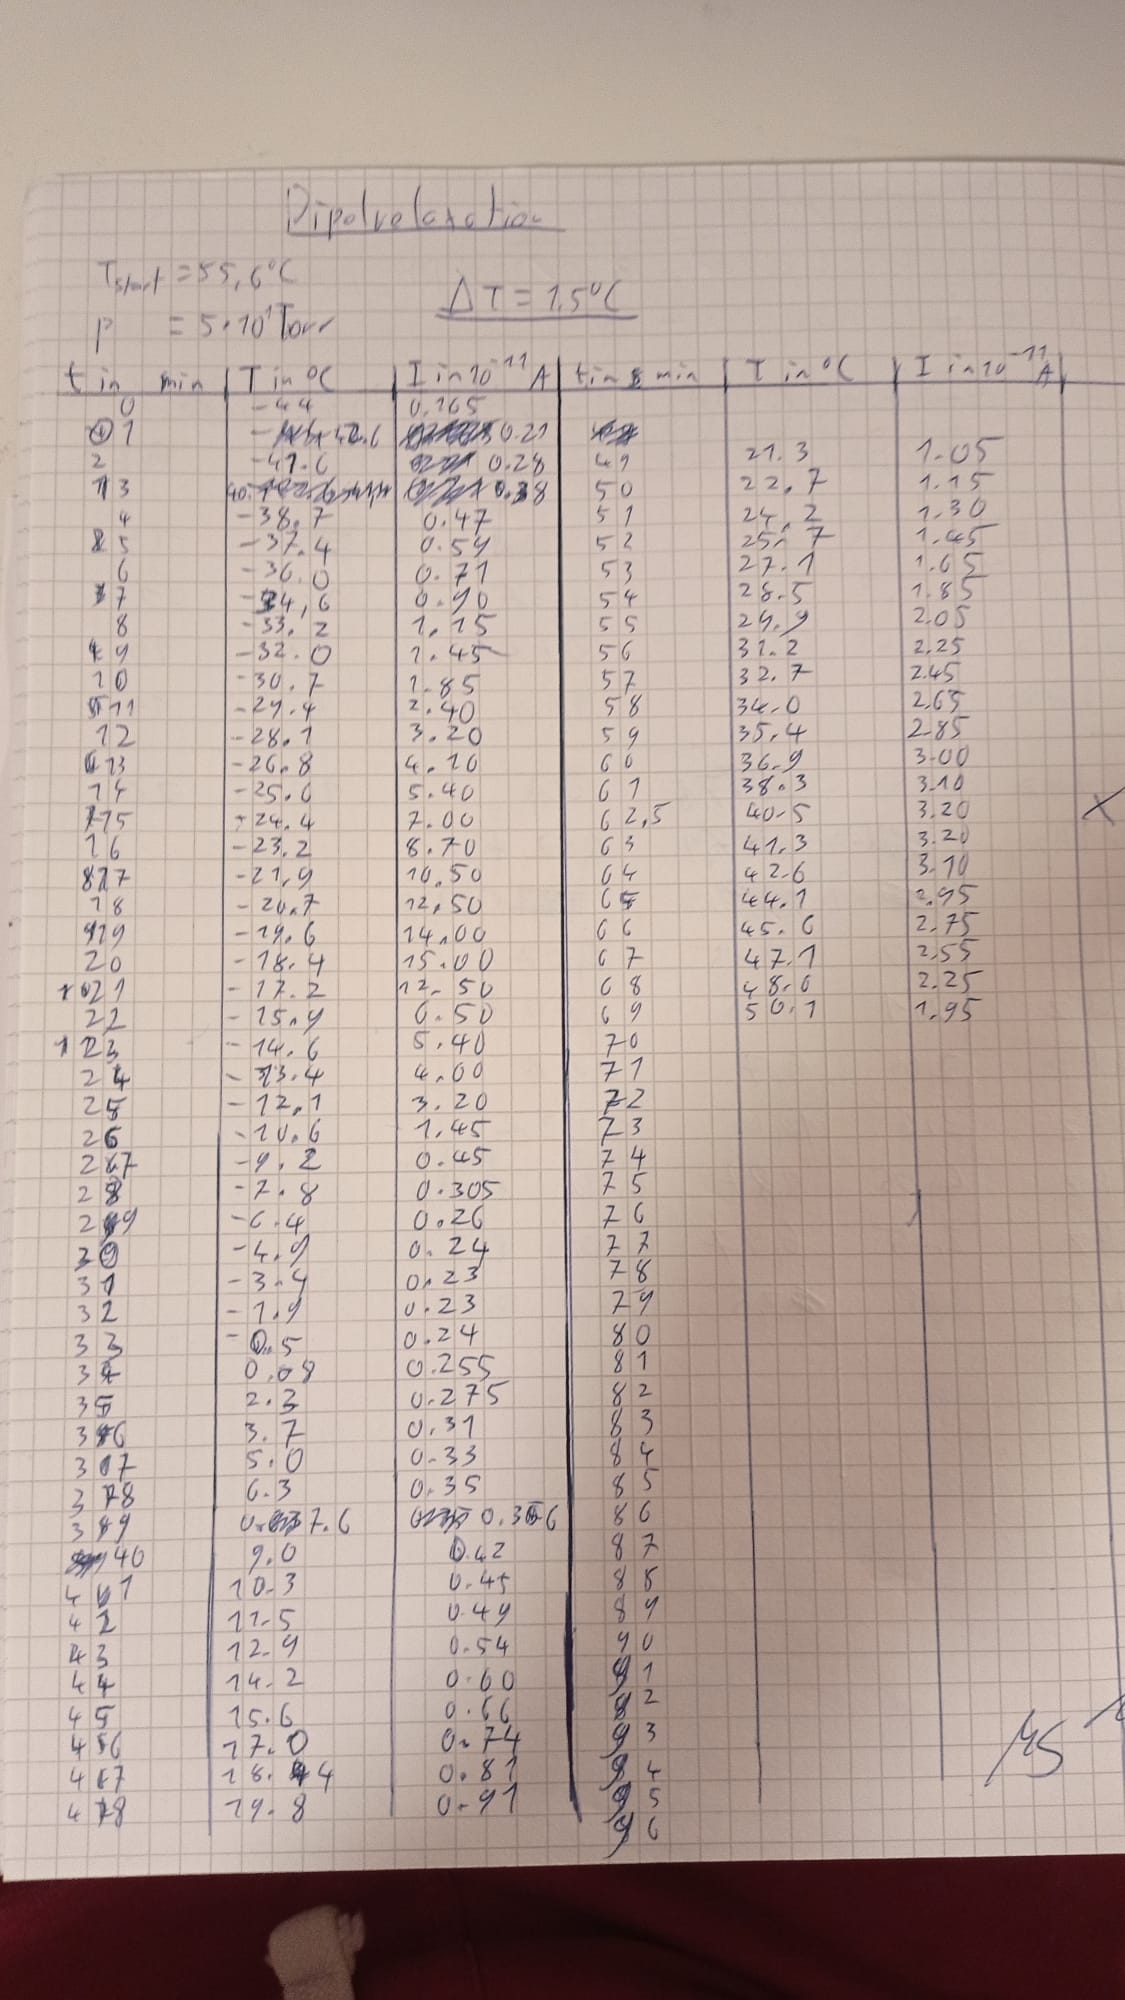
\includegraphics[width=0.7\textwidth]{latex/images/Messwerte_1.jpeg}
    \caption{Die Messwerte des Versuchs Dipolrelaxation.}
\end{figure}

\begin{figure}[h]
    \centering
    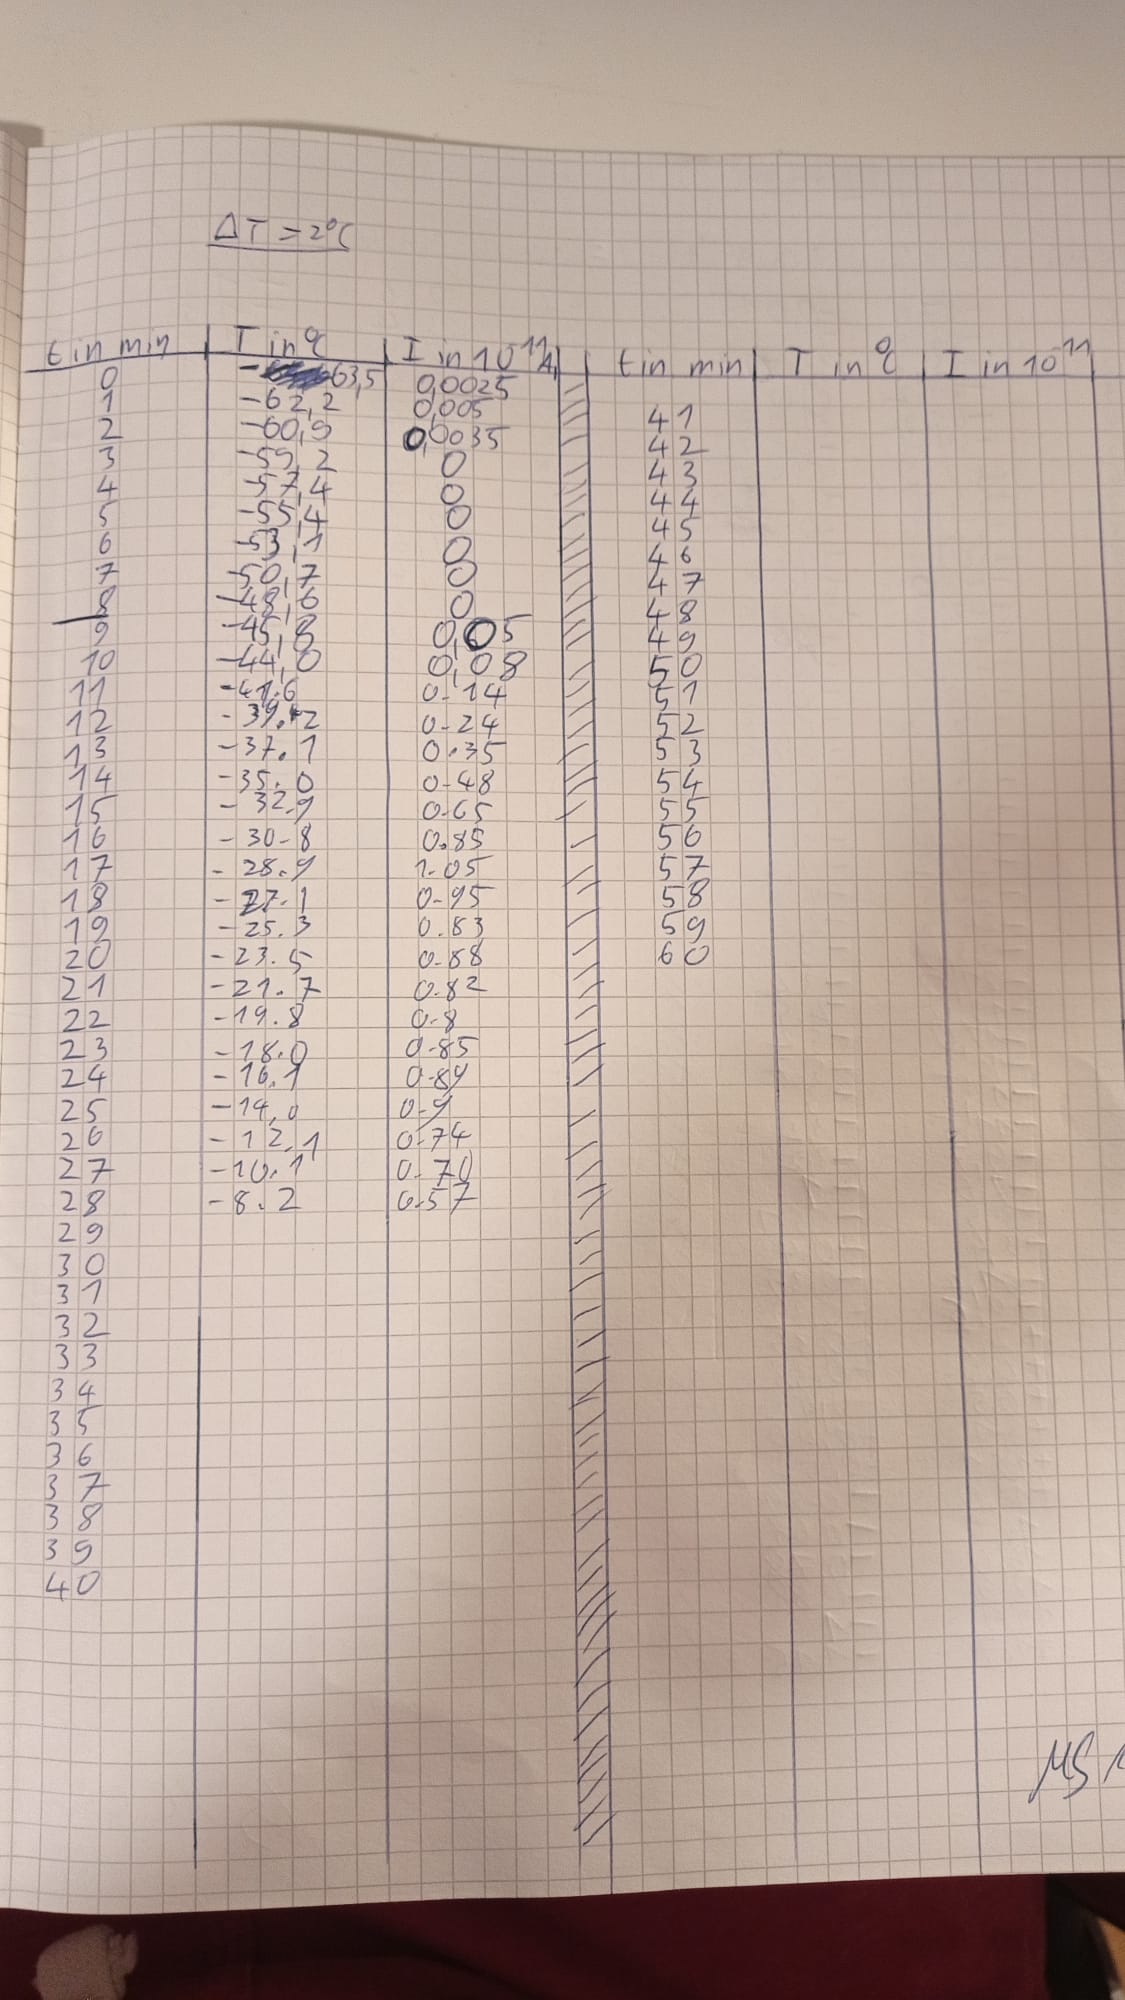
\includegraphics[width=0.7\textwidth]{latex/images/Messwerte_2.jpeg}
    \caption{Die Messwerte des Versuchs Dipolrelaxation.}
\end{figure}

\begin{figure}[h]
    \centering
    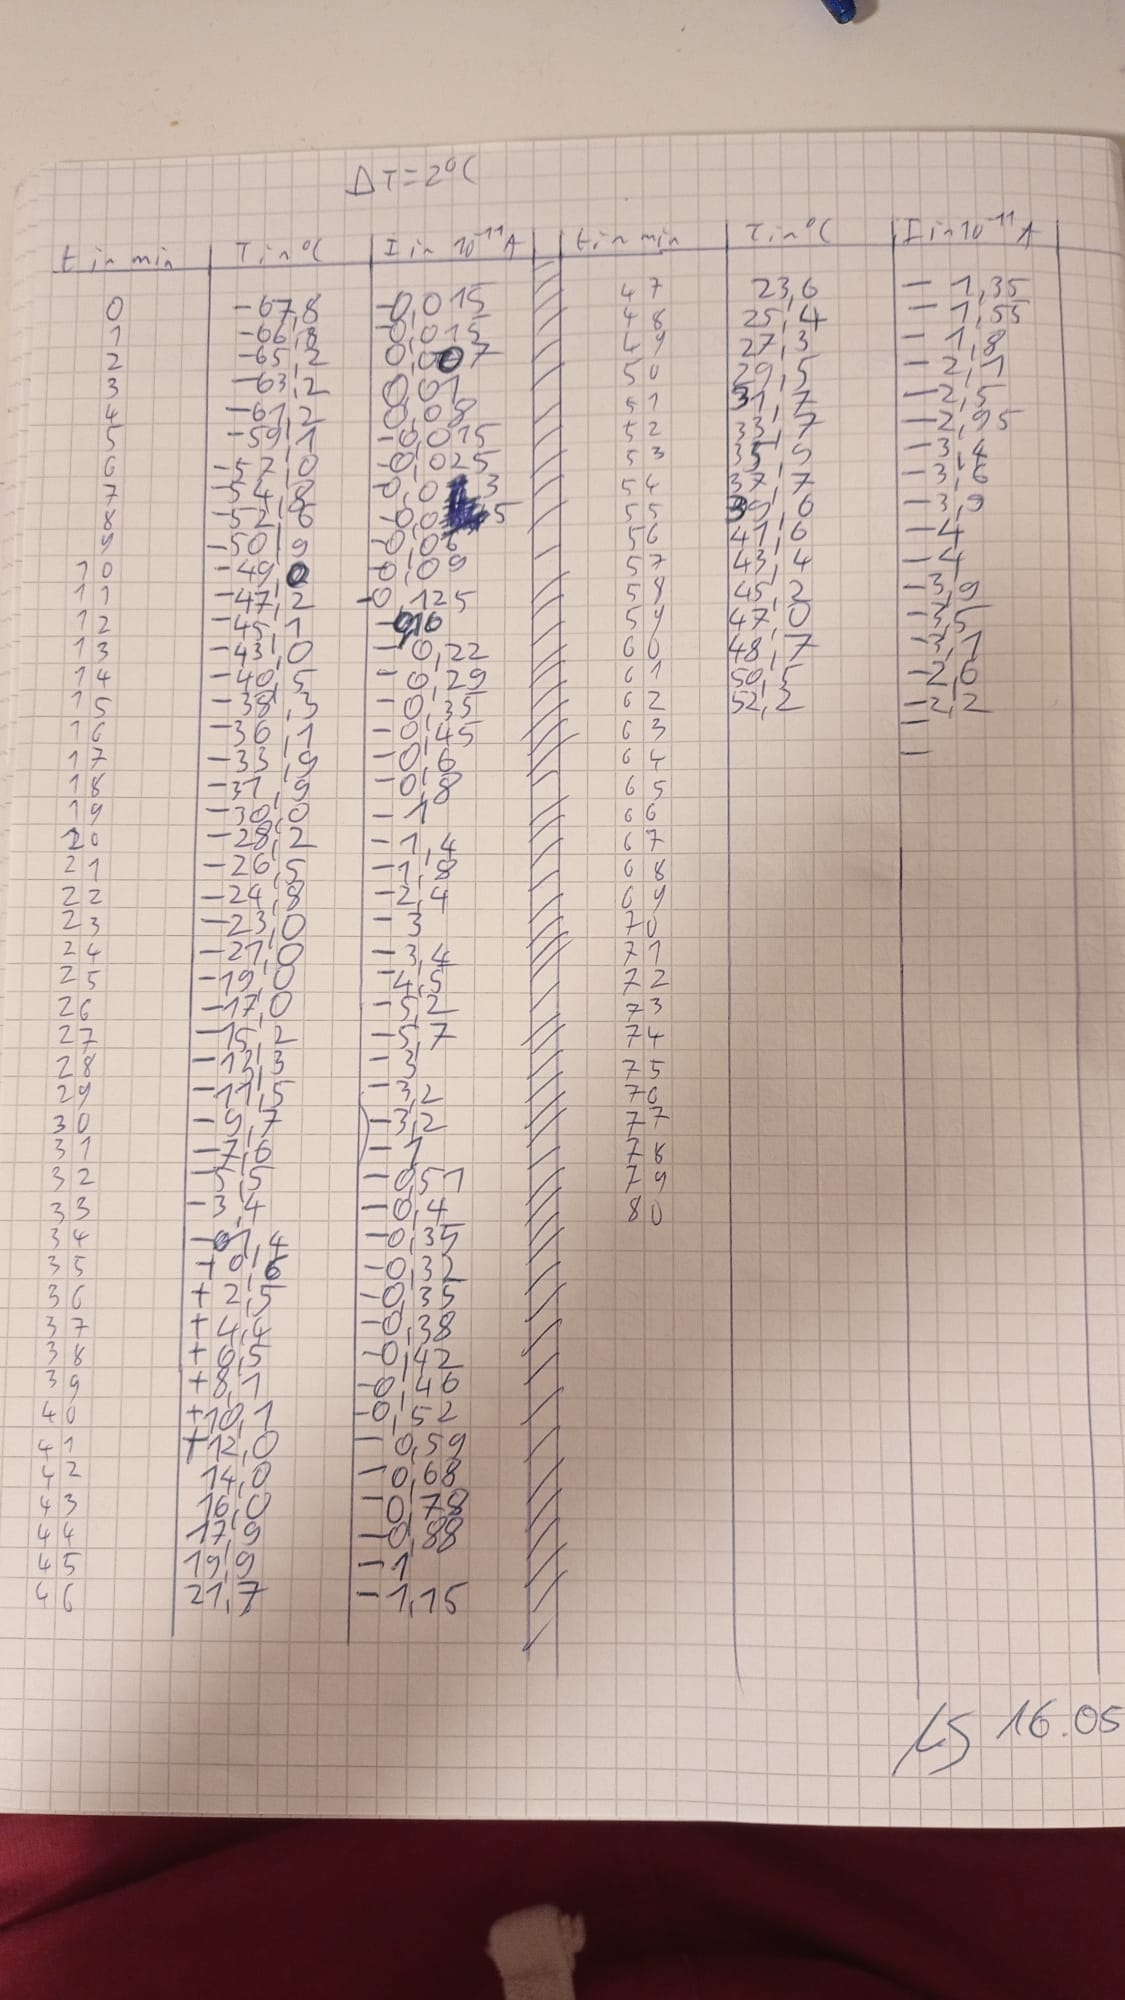
\includegraphics[width=0.7\textwidth]{latex/images/Messwerte_3.jpeg}
    \caption{Die Messwerte des Versuchs Dipolrelaxation.}
\end{figure}
